The preparatory work for this project splits into two parts:
\begin{itemize}
\item Setting up and learning to use the software environment for development. This is described
    in section~\ref{softwarePreparation}.
\item Surveying literature, learning the theoretical background and understanding the existing
    algorithms for my task. The outcome of this preparation shall be discussed first.
\end{itemize}

\section{Rigid body dynamics}
On a most theoretical level, a rigid body is a collection of $k$ point masses ($k \ge 3$) subject
to the constraint that the distance between any pair of masses must remain constant. More
conveniently, we can regard a rigid body as an object with a three-dimensional shape, a non-zero
volume and some mass distribution, and constrain it not to change shape.

At a particular point in time, a rigid body is fully determined by four quantities: the
\emph{position} of its centre of mass, its \emph{orientation}, and its \emph{linear} and
\emph{angular velocities}. These values usually change over time. Each of these can be easily
represented as a three-component vector, except for orientation, which is discussed in
section~\ref{quaternions}. By convention a right-handed Cartesian coordinate system will be used.

To characterize the body's dynamic behaviour, we also need to know its \emph{inertial mass},
a scalar quantity, and its \emph{moment of inertia}, which is a rank-2 tensor (commonly written
as a $3\times3$ matrix). While the mass stays constant, the moment of inertia may
depend on the body's orientation~-- it is, however, constant when expressed with respect to the
body's \emph{principal axes}~\cite{Feynman:63,Goldstein:80}.

Angular velocity appears to be a straightforward way of describing the body's rotation: the
direction of the vector gives the axis of rotation, while its magnitude is the rate of rotation
(most commonly given in radians per second). Unfortunately, in an asymmetric body, the angular
velocity may vary over time even if there are no external influences on the body. It is therefore
sometimes more convenient to use \emph{angular momentum} instead, which is conserved in the
absence of torques.

\begin{table}
\renewcommand{\baselinestretch}{1.3}\small\normalsize
\centerline{\begin{tabular}{|l|l|l|}\hline
& \emph{Linear} & \emph{Angular} \\\hline
Resistance to change & Mass $m$ & Moment of inertia \m{I} \\\hline
Stationary state & Centre of mass position \ve{r} & \emph{see section \ref{quaternions}} \\\hline
Velocity & Linear velocity $\ve{v} = \dot{\ve{r}}$ & Angular velocity \ve{\omega} \\\hline
Momentum & Linear momentum     & Angular momentum           \\
         & $\ve{p} = m\ve{v}$ & $\ve{L} = \m{I}\ve{\omega}$\\\hline
External influence & Force $\ve{F} = \dot{\ve{p}}$ & Torque $\ve{\tau} = \dot{\ve{L}}$ \\\hline
\end{tabular}}
\caption{Summary of the physical quantities describing a rigid body\label{rigidBodySummary}}
\end{table}

Forces and torques acting on a body may change the momenta of a body as described in
table~\ref{rigidBodySummary}. A force \ve{F} may be applied to any point $\ve{r}'$ of
a body. We can treat this as if the force had been applied to the centre of mass \ve{r}, and add
an additional torque given by $\ve{\tau} = (\ve{r}' - \ve{r})\times\ve{F}$. If multiple
forces and torques are applied, all forces (applied to the centre of mass) may be added into
a single vector, and similarly all torques may be added.

To solve the differential equations of motion, forces are integrated over time to find linear
momentum, and torques are integrated to find angular momentum. From each of these we calculate
linear and angular velocities, which are in turn integrated to find the position and orientation
over the course of time. It is important that we integrate over torques (and not angular
accelerations), otherwise the simulation will not correctly conserve angular momentum.

\section{Solving ordinary differential equations (ODEs)}

Undergraduate mathematics courses provide the sufficiently patient student with a range of
different methods for solving ODEs analytically. These work well for simple systems and deliver
an exact answer. For example, if a constant force is applied to a body, its displacement is a
quadratic (parabolic) function of time; if the force is inversely proportional to the
displacement, we get simple harmonic oscillation. Unfortunately, when it the systems become
only slightly more complicated, the equations become intractable~-- even a simple pendulum
already falls in this category. Solutions for these systems can in general only be approximated
numerically.

\begin{figure}
\centerline{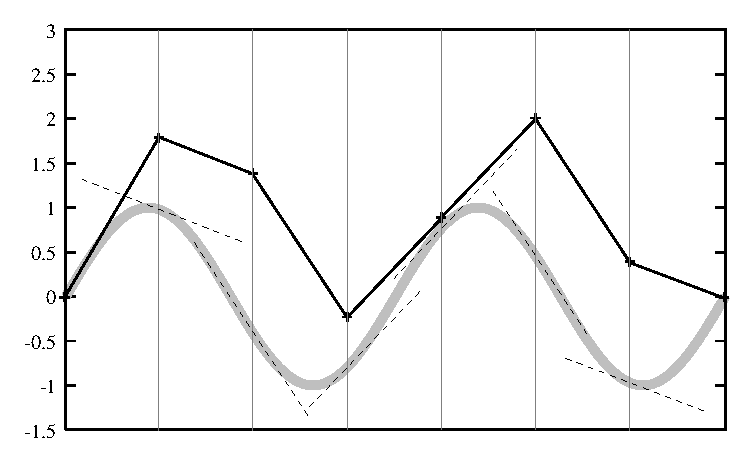
\includegraphics{figures/euler}}
\caption{Demonstration of Euler's method for solving the ODE of simple harmonic oscillation.
    The broad grey line represents the exact solution. At each time step, the method takes the
    derivative (gradient) of the function and uses it to extrapolate linearly.\label{eulersMethod}}
\end{figure}

The general scheme for numerical ODE solvers is to take the value of a function $f(t')$ and its
derivative $\frac{\diff f}{\diff t}(t')$ at some point in time $t'$. From these the algorithm
extrapolates what the value of the function is expected to be some time step $h$ later. The
simplest, most frequently-quoted and worst algorithm for this purpose is Euler's method,
\begin{equation}
f(t'+h) = f(t') + h\frac{\diff f}{\diff t}(t'),
\end{equation}
which performs linear extrapolation. Figure~\ref{eulersMethod} illustrates its operation. The
errors become smaller for tiny time steps, but the method still has a tendency of gaining energy
and is therefore unreliable.
